\chapter{Marco Teórico y Referencial}\label{chapter:marco-teorico-referencial}

El presente capítulo tiene como objetivo analizar los fundamentos teóricos, tecnológicos y los sistemas existentes relacionados con la farmacovigilancia digital y el desarrollo de plataformas de autorreporte clínico. 
Se aborda el estudio de soluciones implementadas a nivel internacional, así como las tecnologías y estándares utilizados en sistemas de salud digital, con el propósito de establecer una base sólida que sustente el diseño e implementación del sistema propuesto.
Asimismo, se revisan conceptos relacionados con el modelado de datos clínicos y estándares de interoperabilidad que garantizan la consistencia y calidad de la información.


\section{Marco Teórico (Fundamentos conceptuales y tecnológicos)}

\subsection{Metodología de desarrollo de software}

Una metodología de desarrollo de software constituye un marco de trabajo estructurado que organiza, planifica y controla el proceso de construcción de un sistema. 
Su relevancia radica en que permite reducir la complejidad del desarrollo al dividir el proyecto en etapas gestionables, establecer un lenguaje común entre los involucrados y mejorar la calidad del producto final mediante prácticas sistemáticas de ingeniería de software \cite{Pfleeger2015}.

En este contexto, existen diversas metodologías de desarrollo, cada una con enfoques particulares para la gestión del ciclo de vida del software.

\begin{itemize}

\item El modelo en cascada sigue un enfoque secuencial y lineal del desarrollo, donde las fases de análisis, diseño, implementación, pruebas y mantenimiento transcurren de manera ordenada y progresiva. Cada fase debe completarse antes de iniciar la siguiente, lo que proporciona un alto nivel de control y documentación, aunque limita la flexibilidad ante cambios durante el desarrollo \cite{Sommerville2015, Royce1987}.

\item Scrum es un marco de trabajo ágil basado en el desarrollo iterativo e incremental. 
El equipo construye el sistema mediante ciclos cortos llamados \textit{sprints}, que producen un incremento funcional del producto al final de cada iteración. 
Scrum define tres artefactos fundamentales para organizar el trabajo y garantizar la calidad: 
\begin{itemize}
    \item La \textit{Pila de Producto} (Product Backlog), lista viva y priorizada de todo lo que el producto necesita, gestionada por el Dueño de Producto (Product Owner).
    \item La \textit{Pila del Sprint} (Sprint Backlog), subconjunto de elementos seleccionados para el sprint en curso junto con el plan para alcanzar el Objetivo del Sprint; 
    \item La \textit{Definición de Terminado} (Definition of Done), que establece los criterios de calidad que un incremento debe cumplir para considerarse finalizado y potencialmente entregable.
\end{itemize}

Scrum define tres roles: el Dueño de Producto, el Scrum Master —facilitador del proceso y encargado de eliminar impedimentos— y el Equipo de Desarrollo. Este marco permite la adaptación continua a cambios mediante eventos como la planificación del sprint, la reunión diaria, la revisión y la retrospectiva \cite{Schwaber2020}.

\item Kanban es un método de gestión del flujo de trabajo orientado a la mejora continua del proceso de desarrollo. Visualiza el trabajo mediante un tablero, limita el trabajo en curso y optimiza el flujo de tareas, permitiendo una entrega continua sin necesidad de iteraciones fijas \cite{Anderson2010}.

\item Extreme Programming (XP) es una metodología ágil centrada en la excelencia técnica del software. Sus valores fundamentales son la simplicidad, la comunicación y la retroalimentación constante. Propone prácticas como el desarrollo guiado por pruebas —que consiste en escribir las pruebas antes del código para verificar su funcionamiento—, la refactorización continua, la programación en parejas, la integración continua y las entregas frecuentes. 
Estas prácticas guardan una relación de complemento mutuo. Juntas buscan reducir los costos del cambio a lo largo del ciclo de vida del proyecto \cite{Beck2004}.

\end{itemize}


\subsubsection{Comparación de metodologías de desarrollo aplicadas al sistema}
\label{subsection:comparacion_metodologias_sistema}

Para seleccionar la metodología más adecuada para el desarrollo del sistema de autorreporte de ESAVI, este análisis comparativo evalúa los diferentes enfoques de desarrollo de software frente a las características específicas del proyecto. La Tabla \ref{tab:comparacion_metodologias_4criterios} sintetiza esta comparación.

Los criterios analizados incluyen la flexibilidad ante cambios de requisitos, la calidad y mantenibilidad del código resultante, el soporte para una arquitectura modular y la adecuación al contexto de desarrollo individual con restricciones operativas como cortes de energía eléctrica y problemas de conectividad.


\begin{table}[h!]
\centering
\renewcommand{\arraystretch}{1.3}
\begin{tabular}{|p{3.5cm}|p{2.8cm}|p{2.8cm}|p{2.8cm}|p{2.8cm}|}
\hline
\textbf{Criterio} & \textbf{Cascada} & \textbf{Scrum} & \textbf{Kanban} & \textbf{XP} \\
\hline

Flexibilidad ante cambios de requisitos y rediseño 
& Baja. Enfoque secuencial con poca capacidad de adaptación una vez avanzadas las fases. 
& Alta. Permite adaptación iterativa de requisitos y ajustes entre entregas. 
& Alta. Facilita la reorganización continua de tareas y prioridades. 
& Alta. Soporta cambios mediante refactorización continua y desarrollo incremental. \\
\hline

Calidad y mantenibilidad del código 
& Baja. No incorpora prácticas técnicas específicas de calidad. 
& Media. Depende de las prácticas del equipo de desarrollo. 
& Baja. No influye directamente en la calidad del código. 
& Alta. Promueve refactorización, simplicidad y buenas prácticas de desarrollo. \\
\hline

Soporte para arquitectura modular (Clean Architecture) 
& Baja. Diseño rígido definido al inicio con poca adaptabilidad. 
& Alta. Permite evolución progresiva de la arquitectura. 
& Media. No define estructura arquitectónica. 
& Alta. Favorece la separación de responsabilidades y modularidad del sistema. \\
\hline

Adecuación al contexto de desarrollo individual y restricciones operativas 
& Baja. Requiere planificación rígida y secuencial. 
& Media. Diseñado para equipos, requiere adaptación en contexto individual. 
& Alta. Flexible y adecuado para gestión individual de tareas. 
& Alta. Compatible con desarrollo individual y mejora continua del código. \\
\hline

\end{tabular}
\caption{Comparación de metodologías de desarrollo según criterios del sistema}
\label{tab:comparacion_metodologias_4criterios}
\end{table}

\subsection{Patrones de diseño de software}

\subsection{Fundamentos de bases de datos}

% que es acid, que es modelo relacional, que es normalización

\subsection{Análisis de tecnologías para la implementación del sistema propuesto}

\subsubsection{Tecnologías de backend}

\subsubsection{Tecnologías de frontend}

\subsubsection{Sistemas de gestión de bases de datos}

\subsection{Otras herramientas y librerías}



\section{Marco Referencial (Estado del Arte)}

\subsection{Limitaciones de plataformas genéricas (Google Forms)}

El uso de plataformas de formularios en la nube como Google Forms, Microsoft Forms o JotForm podría considerarse una alternativa rápida para la captura de eventos adversos. Sin embargo, sus características las inhabilitan como solución para un sistema nacional de farmacovigilancia:

\begin{itemize}

\item \textbf{Soberanía de los datos:} La información de salud se almacena en servidores externos bajo jurisdicciones extranjeras, vulnerando el principio de residencia de datos clínicos que exige el marco regulatorio nacional.

\item \textbf{Validación clínica insuficiente:} Solo ofrecen validaciones básicas (campos obligatorios, formatos). Carecen de capacidad para integrar codificación clínica estandarizada o para implementar reglas de negocio complejas como la coherencia cronológica entre vacunación y aparición de síntomas.

\item \textbf{Ausencia de control de acceso granular:} No permiten definir roles diferenciados (reportante, médico evaluador, jefe de vacunación) con permisos específicos, lo cual es indispensable en un flujo de farmacovigilancia.

\item \textbf{Falta de trazabilidad:} No registran quién modificó un reporte ni cuándo, imposibilitando la auditoría de los datos.

\item \textbf{Interoperabilidad nula:} Los datos se exportan manualmente a hojas de cálculo, impidiendo la integración automatizada con sistemas de información de salud.

\end{itemize}

En consecuencia, estas plataformas son adecuadas para encuestas, pero no para un sistema de autorreporte de ESAVI que requiere seguridad, estructuración, trazabilidad e interoperabilidad. Esta brecha justifica el desarrollo de una solución específica.

\subsection{Análisis de sistemas de autorreporte de eventos adversos existentes}

En la farmacovigilancia moderna, los sistemas de autorreporte clínico permiten registrar eventos adversos posteriores a la vacunación de forma estructurada. 
Estas herramientas operan bajo dos modelos principales: la vigilancia pasiva y la vigilancia activa. El modelo pasivo depende exclusivamente de la iniciativa voluntaria de ciudadanos o profesionales para notificar un evento.
Por el contrario, el modelo activo o proactivo establece un contacto directo con el usuario mediante encuestas digitales para recopilar datos de salud en tiempo casi real.

Este apartado examina tres sistemas representativos a nivel internacional —VAERS, NotificaRAM y V-safe— con el objetivo de identificar brechas de diseño que fundamenten la propuesta del sistema ESAVI del IFV.

\subsubsection{Vaccine Adverse Event Reporting System (VAERS)}

\textbf{VAERS} es el sistema nacional de farmacovigilancia en los Estados Unidos, administrado por la \textit{Food and Drug Administration} (FDA), agencia reguladora de medicamentos y alimentos, y los \textit{Centers for Disease Control and Prevention} (CDC), organismo responsable del control y prevención de enfermedades \cite{fda_vaers}. 
Su objetivo principal es detectar señales de seguridad no identificados durante los ensayos clínicos \cite{cdc_vaers}.

Permite la notificación voluntaria de eventos adversos por parte de profesionales de la salud, fabricantes y ciudadanos mediante formularios web y PDF descargables \cite{vaers_official}.
Para garantizar la integridad del repositorio, la legislación estadounidense contempla sanciones civiles y penales ante el suministro intencional de información falsa en los reportes \cite{vaers_official}. 
Esto contribuye a reducir la introducción de datos malintencionados en un sistema de acceso público.

Los reportes alimentan la base de datos CDC WONDER\footnote{CDC WONDER (Wide-ranging Online Data for Epidemiologic Research): plataforma de los CDC para el acceso público a datos epidemiológicos anonimizados.}, garantizando la transparencia mediante su disponibilidad abierta \cite{vaers_official}. 
Ante una señal de alerta, el monitoreo escala hacia sistemas complementarios de vigilancia activa y evaluación clínica como VSD\footnote{Vaccine Safety Datalink (VSD): red de vigilancia que integra datos de múltiples organizaciones sanitarias para el análisis de seguridad vacunal.} y el proyecto CISA\footnote{Clinical Immunization Safety Assessment (CISA): iniciativa orientada a la evaluación clínica especializada de eventos adversos asociados a la vacunación.} para confirmar posibles riesgos \cite{cdc_vaers}.

\subsubsection{NotificaRAM}

\textbf{NotificaRAM} es la plataforma oficial de farmacovigilancia en España para la notificación de sospechas de reacciones adversas a medicamentos \cite{aemps_manual_2025}.
\textit{La Agencia Española de Medicamentos y Productos Sanitarios (AEMPS)} gestiona este portal en el marco del Sistema Español de Farmacovigilancia de Medicamentos de Uso Humano (SEFV-H) \cite{aemps_sefv_2025}.

El sistema funciona de forma descentralizada, remitiendo los reportes a los Centros Autonómicos de Farmacovigilancia para su validación técnica inicial \cite{aemps_manual_2025}. 
Tras esta evaluación, la base de datos \textit{FEDRA(Farmacovigilancia Española, Datos de Reacciones Adversas)}, sistema nacional de notificación y almacenamiento de sospechas de reacciones adversas a medicamentos en España, centraliza todos los registros del país \cite{aemps_fedra_2026}.
Estos registros alimentan la plataforma europea \textit{EudraVigilance}, sistema de la Agencia Europea de Medicamentos (EMA) destinado a la gestión y análisis de notificaciones de sospechas de reacciones adversas a medicamentos, utilizada por las agencias reguladoras de la Unión Europea para la detección de señales de seguridad.

Finalmente, la base de datos global \textit{VigiBase}, gestionada por el \textit{Centro de Monitoreo de Uppsala bajo la Organización Mundial de la Salud (OMS)}, consolida reportes de seguridad a nivel mundial para el monitoreo internacional de eventos adversos \cite{aemps_notificacion_2026}.


\subsubsection{V-safe}


Los Centers for Disease Control and Prevention (CDC) diseñaron \textbf{V-safe} como una herramienta digital para monitorear la seguridad vacunal en los Estados Unidos.
Tras su lanzamiento inicial en diciembre de 2020 para supervisar las vacunas contra la COVID-19, el sistema extendió su alcance a otras inmunizaciones, incluyendo aquellas contra el virus respiratorio sincitial (VRS) \cite{cdc_vsafe_portal}.

A diferencia de los modelos de notificación espontánea, V-safe emplea un enfoque de vigilancia activa mediante el contacto proactivo con los usuarios. 
El sistema envía encuestas digitales por mensajes de texto o correo electrónico para recopilar información directamente del paciente \cite{cdc_about_vsafe}.
El sistema realiza el seguimiento mediante encuestas diarias durante la primera semana posterior a la vacunación y, posteriormente, mediante encuestas semanales durante seis semanas adicionales \cite{cdc_vsafe_portal,vsafe_monitoring_article}.

La Figura \ref{fig:vsafe_flujo} ilustra el flujo general de interacción del sistema, basado en el envío periódico de encuestas y la recopilación estructurada de datos reportados por los usuarios \cite{vsafe_monitoring_article}.

\begin{figure}[H]
    \centering
    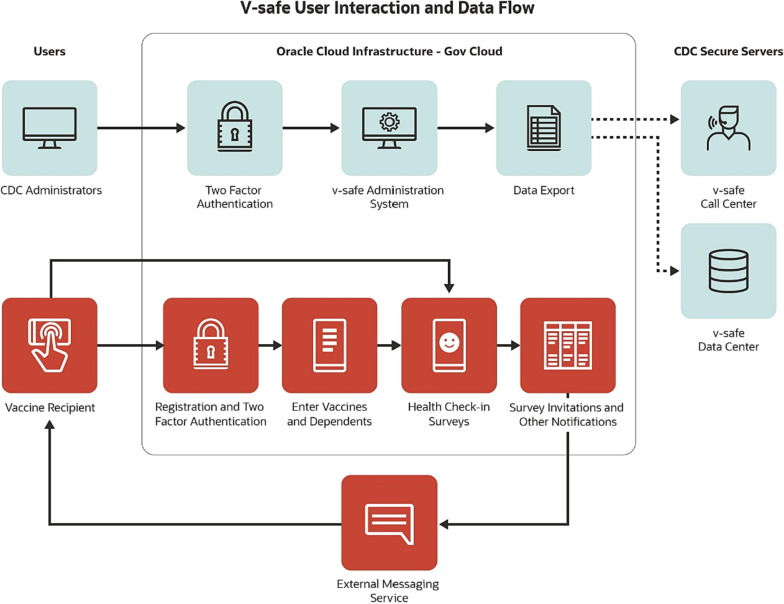
\includegraphics[scale=2.5]{Graphics/gr1_lrg.jpg}
    \caption{Ejemplo del flujo de interacción del sistema V-safe mediante encuestas digitales}
    \label{fig:vsafe_flujo}
\end{figure}

El funcionamiento detallado de la interfaz de usuario del sistema V-safe puede observarse en el Anexo~\ref{app:vsafe-form-ene2021}, donde se presentan capturas representativas del flujo de interacción, que muestran el reporte rápido, estructurado y de baja carga del estado de salud diario del usuario.

V-safe integra sistemas de vigilancia pasiva: cuando un usuario reporta la necesidad de atención médica, el sistema facilita la generación de un reporte en VAERS mediante la precarga de datos \cite{cdc_about_vsafe}.
Además, la plataforma publica los datos recopilados en formato anonimizado para su consulta en portales de acceso público.

\subsection{Análisis comparativo de los sistemas estudiados}

Este análisis compara los sistemas VAERS, V-safe y NotificaRAM en términos de su enfoque metodológico, grado de digitalización y mecanismos de captura de datos. La Tabla \ref{tab:sistemas_comparacion} sintetiza estos criterios con el objetivo de evidenciar diferencias estructurales en los modelos actuales de farmacovigilancia.


\begin{table}[htbp]
	\centering
	\caption{Comparación de sistemas de autorreporte de eventos adversos}
	\label{tab:sistemas_comparacion}
	
	\renewcommand{\arraystretch}{1.3}
	
	\begin{tabular}{p{3.2cm} p{4.3cm} p{4.3cm} p{4.3cm}}
		
		\textbf{Criterio} & \textbf{VAERS} & \textbf{NotificaRAM} & \textbf{V-safe} \\[6pt]
		
		Tipo de vigilancia &
		Pasiva  &
		Pasiva  &
		Activa  \\[6pt]
		\hline

		Actores &
		Profesionales de salud, fabricantes y ciudadanos &
		Profesionales de salud y ciudadanos &
		Usuarios vacunados registrados \\[6pt]
        \hline
		
		Canal de notificación &
		Formularios web y PDF descargables &
		Formulario electrónico nacional &
		Encuestas digitales (SMS y correo electrónico) \\[6pt]
        \hline
		
		Protección de datos &
		Datos anonimizados accesibles vía CDC WONDER &
		Marco europeo de protección de datos \cite{aemps_fedra_2026} &
		Datos \gls{desidentificados} bajo políticas federales \\[6pt]
        \hline
		
		Estructuración del dato &
		Predominio de texto libre; baja estandarización &
		Formularios con campos definidos; control parcial &
		Formularios digitales con validación y opciones predefinidas
		\\[6pt]
        \hline
		
	
	Fortalezas
	& Alta cobertura poblacional; acceso público a los datos; detección temprana de señales  
	& Integración en red nacional de farmacovigilancia; análisis coordinado; interoperabilidad con sistemas europeos  
	& Recolección sistemática y periódica; datos en tiempo casi real; seguimiento longitudinal  \\[6pt]
    \hline
	
	
	Limitaciones
	& Subregistro; sesgos de notificación; calidad variable de los datos; no permite establecer causalidad directa
	& Subregistro; dependencia de la iniciativa del notificador; variabilidad en la calidad de los datos
	& Dependencia de acceso a tecnología; participación voluntaria; posible fatiga del usuario; limitada representatividad
    

	\end{tabular}
\end{table}




\subsection{Síntesis de brechas y requerimientos para ESAVI-Cuba}





\section{Conclusiones del capítulo}
\label{section:conclusiones_estado_arte}

